% !TeX program = xelatex
% Roll-up poster, EFA 2026. Visible size 700 x 2000 mm + 5 mm bleed -> 710 x 2010 mm.
%
% IMPORTANT: compile with XeLaTeX (or LuaLaTeX), NOT pdfLaTeX.
% On Overleaf: Menu (top left) -> Compiler -> XeLaTeX.
% Needs the Figures/ folder from the repo next to this file.
%
% Print-ready step (text outlined, CMYK, no crop marks) after compiling:
%   gs -dBATCH -dNOPAUSE -sDEVICE=pdfwrite -dCompatibilityLevel=1.4 -dNoOutputFonts \
%      -sColorConversionStrategy=CMYK -dProcessColorModel=/DeviceCMYK \
%      -dDownsampleColorImages=false -dAutoFilterColorImages=false -dColorImageFilter=/FlateEncode \
%      -o Hermes_EFA_poster_print.pdf poster_EFA.pdf
\documentclass{article}

\usepackage[paperwidth=710mm,paperheight=2010mm,left=45mm,right=45mm,top=0mm,bottom=0mm]{geometry}
\usepackage[cmyk]{xcolor}
\usepackage{graphicx}
\usepackage{amsmath}
\usepackage{amssymb}
\usepackage{lmodern}
\usepackage{booktabs}
\usepackage{array}
\usepackage{enumitem}
\usepackage{tikz}
\usetikzlibrary{positioning,arrows.meta}
\usepackage[most]{tcolorbox}
\usepackage{iftex}
\ifPDFTeX
  \errmessage{Compile this poster with XeLaTeX or LuaLaTeX, not pdfLaTeX. On Overleaf: Menu -> Compiler -> XeLaTeX}
\fi
\usepackage{fontspec}
\IfFontExistsTF{Lato}
  {\setmainfont{Lato}[BoldFont={Lato Bold},ItalicFont={Lato Italic}]}
  {\IfFontExistsTF{Lato-Regular.ttf}
    {\setmainfont{Lato-Regular.ttf}[BoldFont=Lato-Bold.ttf,ItalicFont=Lato-Italic.ttf]}
    {}}% falls back to the default font, still compiles
\IfFontExistsTF{Lato Black}
  {\newfontfamily\LatoBlack{Lato Black}}
  {\IfFontExistsTF{Lato-Black.ttf}
    {\newfontfamily\LatoBlack{Lato-Black.ttf}}
    {\newcommand{\LatoBlack}{\bfseries}}}

% Palette of the slide deck, defined directly in CMYK
\definecolor{navy}{cmyk}{1,0.39,0,0.58}      % #00416A
\definecolor{rust}{cmyk}{0,0.69,0.83,0.23}   % #C43D21
\definecolor{grn}{cmyk}{1,0,0.25,0.50}       % #008060
\definecolor{pale}{cmyk}{0.045,0.025,0,0.043}% #E9EEF4
\definecolor{paleg}{cmyk}{0.06,0,0.03,0.035}
\definecolor{paler}{cmyk}{0,0.06,0.06,0.015}
\definecolor{midgrey}{cmyk}{0,0,0,0.55}
\definecolor{ink}{cmyk}{0,0,0,0.92}
\definecolor{pagebg}{cmyk}{0.10,0.055,0,0.055}

% Font sizes
\newcommand{\fTitle}{\fontsize{92}{102}\selectfont}
\newcommand{\fSub}{\fontsize{38}{48}\selectfont}
\newcommand{\fSect}{\fontsize{42}{50}\selectfont}
\newcommand{\fHead}{\fontsize{33}{42}\selectfont}
\newcommand{\fBody}{\fontsize{25}{33}\selectfont}
\newcommand{\fTab}{\fontsize{22}{30}\selectfont}
\newcommand{\fSmall}{\fontsize{21}{28}\selectfont}
\newcommand{\fTiny}{\fontsize{17}{22.5}\selectfont}
\newcommand{\fStat}{\fontsize{44}{48}\selectfont}

\setlength{\parindent}{0pt}
\pagestyle{empty}
\color{ink}

\setlist[itemize]{label={\textcolor{navy}{\rule[0.18em]{0.5em}{0.5em}}},leftmargin=1.4em,itemsep=0.35\baselineskip,parsep=0pt,topsep=0.25\baselineskip}

\pagecolor{pagebg}

\newcommand{\fullbleed}[1]{\noindent\makebox[\textwidth][c]{#1}}

% White section cards on the tinted page background
\newtcolorbox{PanelBox}{enhanced,colback=white,colframe=white,boxrule=0pt,arc=5mm,
  width=644mm,left=12mm,right=12mm,top=8mm,bottom=10mm,nobeforeafter}
\newenvironment{Panel}
  {\par\vspace{9mm plus 4mm}\noindent\hspace*{-12mm}\begin{PanelBox}}
  {\end{PanelBox}\par}

\newcommand{\Section}[1]{%
  {\fSect\bfseries\color{navy}#1\par}
  \vspace{2.5mm}{\color{navy}\rule{\textwidth}{1.5pt}}\par
  \vspace{6mm}}

\newcommand{\Message}[1]{%
  \vspace{4mm}
  {\fHead\color{navy}\raisebox{1pt}{$\blacktriangleright$}\hspace{0.5em}\textbf{#1}\par}}

\newcommand{\FigNote}[1]{\par\vspace{1.5mm}{\fTiny\color{midgrey}#1\par}}

\renewcommand{\arraystretch}{1.15}

\begin{document}

% ============================= HEADER =============================
\fullbleed{%
\begin{tcolorbox}[colback=navy,colframe=navy,sharp corners,boxrule=0pt,
    width=710mm,left=50mm,right=50mm,top=24mm,bottom=16mm]
  \color{white}
  \centering
  {\fTitle\LatoBlack Hedge Fund Trading and\\[3mm] Sovereign Bond Yield Sensitivity\par}
  \vspace{6mm}
  {\fSub\bfseries Felix Hermes\par}
  \vspace{2.5mm}
  {\fSub Goethe University Frankfurt \& European Central Bank\par}
\end{tcolorbox}}

% ======================= MOTIVATION + QUESTION =======================
\begin{Panel}
\Section{Hedge funds hold a growing footprint in government bond markets}

\begin{minipage}[c]{215mm}
  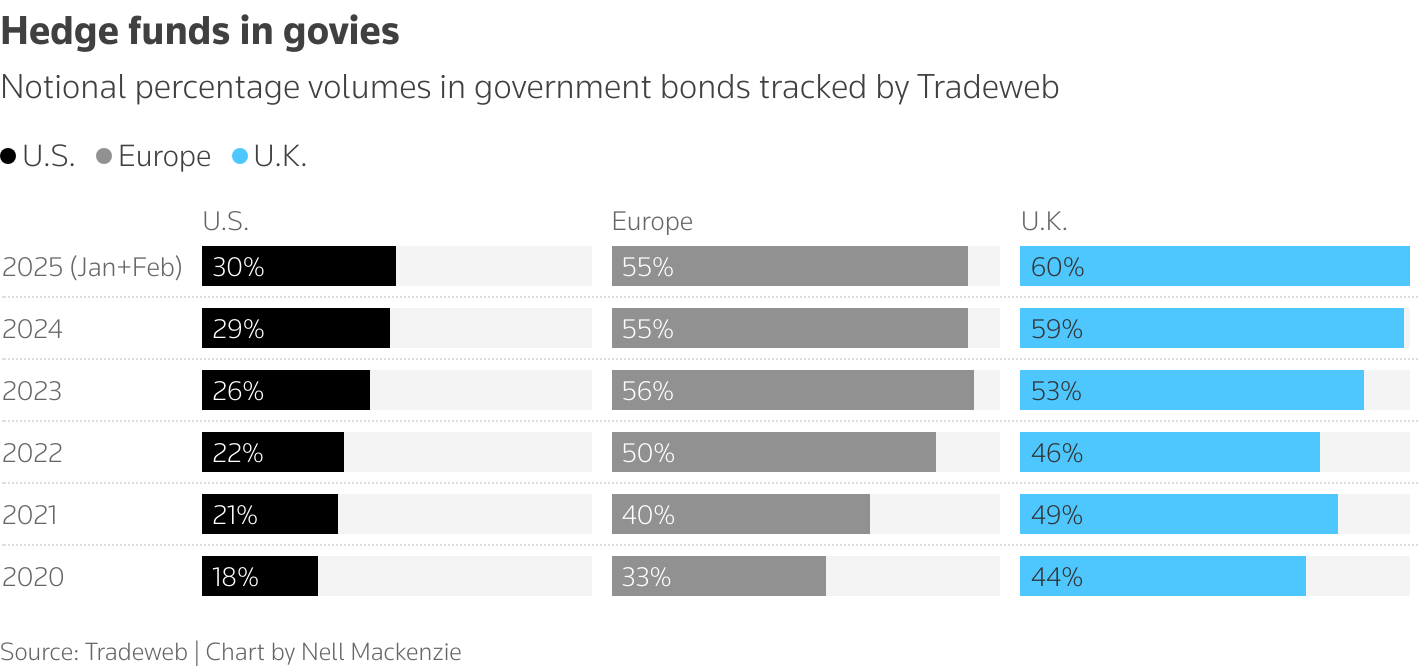
\includegraphics[width=215mm]{Figures/tradeweb.png}
  \FigNote{Hedge fund share of trading volume in government bonds tracked by Tradeweb.}
\end{minipage}\hfill
\begin{minipage}[c]{368mm}\fBody
\begin{itemize}
  \item Since 2020 their share of trading volume in Europe rose from a third to \textbf{more than half}.
  \item Positions are financed in the \textbf{repo market}: leverage ties funding to collateral values.
  \item Granular evidence outside of crises is scarce.
\end{itemize}
\end{minipage}

\vspace{9mm}
\begin{minipage}[t]{302mm}
\begin{tcolorbox}[colback=paleg,colframe=grn,boxrule=1.4pt,arc=3mm,left=7mm,right=7mm,top=3.5mm,bottom=3.5mm]
  \centering{\fHead\bfseries\color{grn}Decrease sensitivity\par}\vspace{2mm}
  {\fBody Arbitrage corrects mispricings.\\Prices are pushed \textit{toward} fundamentals.\par}\vspace{2mm}
  {\fTiny\color{midgrey}Gromb and Vayanos (2002), Cao et al.\ (2018)\par}
\end{tcolorbox}
\end{minipage}\hfill
\begin{minipage}[t]{302mm}
\begin{tcolorbox}[colback=paler,colframe=rust,boxrule=1.4pt,arc=3mm,left=7mm,right=7mm,top=3.5mm,bottom=3.5mm]
  \centering{\fHead\bfseries\color{rust}Increase sensitivity\par}\vspace{2mm}
  {\fBody Leverage and funding fragility force trades.\\Prices are pushed \textit{away} from fundamentals.\par}\vspace{2mm}
  {\fTiny\color{midgrey}Shleifer and Vishny (1997), Brunnermeier and Pedersen (2009)\par}
\end{tcolorbox}
\end{minipage}

\Message{Research question: does the leveraged positioning of hedge funds amplify sovereign bond yield sensitivity to shocks --- and under what conditions?}
\end{Panel}

% ============================== DATA ==============================
\begin{Panel}
\Section{Data and empirical design}

\begin{minipage}[t]{200mm}
  {\fHead\bfseries\color{navy}Hedge fund repo positions\par}\vspace{1.5mm}
  {\fSmall\color{midgrey}ECB SFTDS\par}\vspace{2.5mm}
  {\fBody Transaction-level euro area repo data: German and Italian sovereigns, Jan 2021 -- Nov 2025. 152 offshore hedge funds. Repo $=$ long, reverse repo $=$ short.\par}
\end{minipage}\hfill
\begin{minipage}[t]{195mm}
  {\fHead\bfseries\color{navy}Bond characteristics\par}\vspace{1.5mm}
  {\fSmall\color{midgrey}Bloomberg\par}\vspace{2.5mm}
  {\fBody Daily yields, duration, bid-ask spread, amount issued, and cheapest-to-deliver status per bond.\par}
\end{minipage}\hfill
\begin{minipage}[t]{200mm}
  {\fHead\bfseries\color{navy}Exogenous shocks\par}\vspace{1.5mm}
  {\fSmall\color{midgrey}EA-MPD (Altavilla et al.\ 2019)\par}\vspace{2.5mm}
  {\fBody Intraday 2-year OIS change in the ECB event window: the same shock hits every bond.\par}
\end{minipage}

\vspace{9mm}
\begin{tcolorbox}[colback=pale,colframe=pale,arc=3mm,left=9mm,right=9mm,top=6.5mm,bottom=6.5mm]
  \centering\fBody
  $\Delta y_{i,t} \;=\; {\color{rust}\beta_1\,(\mathrm{HF}_{i,t-1} \times \mathrm{Shock}_{t})} \;+\; \beta_2\, \mathrm{HF}_{i,t-1} \;+\; \beta_3\, \mathrm{Shock}_{t} \;+\; \gamma\, \mathbf{X}_{i,t-1} \;+\; \theta_{k} \;+\; \varepsilon_{i,t}$
  \par\vspace{3.5mm}
  {\fSmall ${\color{rust}\beta_1}$: additional yield sensitivity when hedge funds are positioned --- presence dummy, or intensity (five-day net position / amount outstanding).\par}
\end{tcolorbox}

\vspace{8mm}
\begin{minipage}[c]{330mm}\fBody
  {\fHead\bfseries\color{navy}Identification\par}\vspace{2mm}
\begin{itemize}
  \item Hedge funds select liquid, large, long-duration, cheapest-to-deliver bonds.
  \item Duration $\times$ country $\times$ date FE compare similar bonds of the same issuer on the same day; a matched design pairs each bond with its closest twin.
  \item A dealer-level panel shows the trigger is not dealer behavior.
\end{itemize}
\end{minipage}\hfill
\begin{minipage}[c]{270mm}
\centering
\begin{tabular}{c c}
  {\fStat\bfseries\color{navy}152} & {\fStat\bfseries\color{navy}477{,}001}\\[1mm]
  {\fSmall hedge funds} & {\fSmall bond-days}\\[6mm]
  {\fStat\bfseries\color{navy}38} & {\fStat\bfseries\color{navy}3\%}\\[1mm]
  {\fSmall ECB announcements} & {\fSmall of an issue held when active}\\
\end{tabular}
\end{minipage}
\end{Panel}

% ============================ MECHANISM ============================
\begin{Panel}
\Section{How leveraged positioning amplifies yields}

{\fBody\textbf{Adrian and Shin (2014):} leveraged intermediaries manage their balance sheet against the risk environment --- the same rule produces opposite adjustments depending on the sign of the shock.\par}
\vspace{8mm}

\begin{center}

\begin{tikzpicture}[box/.style={draw=navy,line width=1.3pt,rounded corners=3mm,align=center,inner xsep=7mm,inner ysep=4mm}]
  \node[box,draw=rust,fill=paler] (con)
    {\fHead\bfseries\color{rust}Constraining\\[1mm]\fBody\color{ink} price moves \textit{against} the position\\ capital buffer erodes $\rightarrow$ fund \textbf{reduces} exposure};
  \node[box,fill=pale,right=16mm of con] (top) {\fHead\bfseries\color{navy} Shock meets a pre-determined\\[1mm]\fHead\bfseries\color{navy} leveraged position};
  \node[box,draw=grn,fill=paleg,right=16mm of top] (rel)
    {\fHead\bfseries\color{grn}Relaxing\\[1mm]\fBody\color{ink} price moves \textit{in favor}\\ constraint loosens $\rightarrow$ fund \textbf{expands} exposure};
  \draw[-{Latex[length=5mm]},line width=1.5pt,navy] (top.west) -- (con.east);
  \draw[-{Latex[length=5mm]},line width=1.5pt,navy] (top.east) -- (rel.west);
\end{tikzpicture}
\end{center}

\vspace{6mm}
{\fBody\textbf{\color{navy}Numerical example} (margin 2\%, duration 7y, sector holds 3\% of the issue):\quad 6 bp surprise $\rightarrow$ price $-0.42\%$ $\rightarrow$ capital buffer $\color{rust}\mathbf{-21\%}$ $\rightarrow$ trading pressure $0.63\%$ of the issue $\rightarrow$ $\color{rust}\mathbf{+3.15}$ \textbf{\color{rust}bp} extra yield move.\par}

\Message{In both states the resulting trading pushes yields further in the direction of the initial shock.}
\end{Panel}

% ============================ FINDING 1 ============================
\begin{Panel}
\Section{Finding 1: Hedge funds increase the volatility of bond yields on shock days}

\begin{minipage}[c]{240mm}
  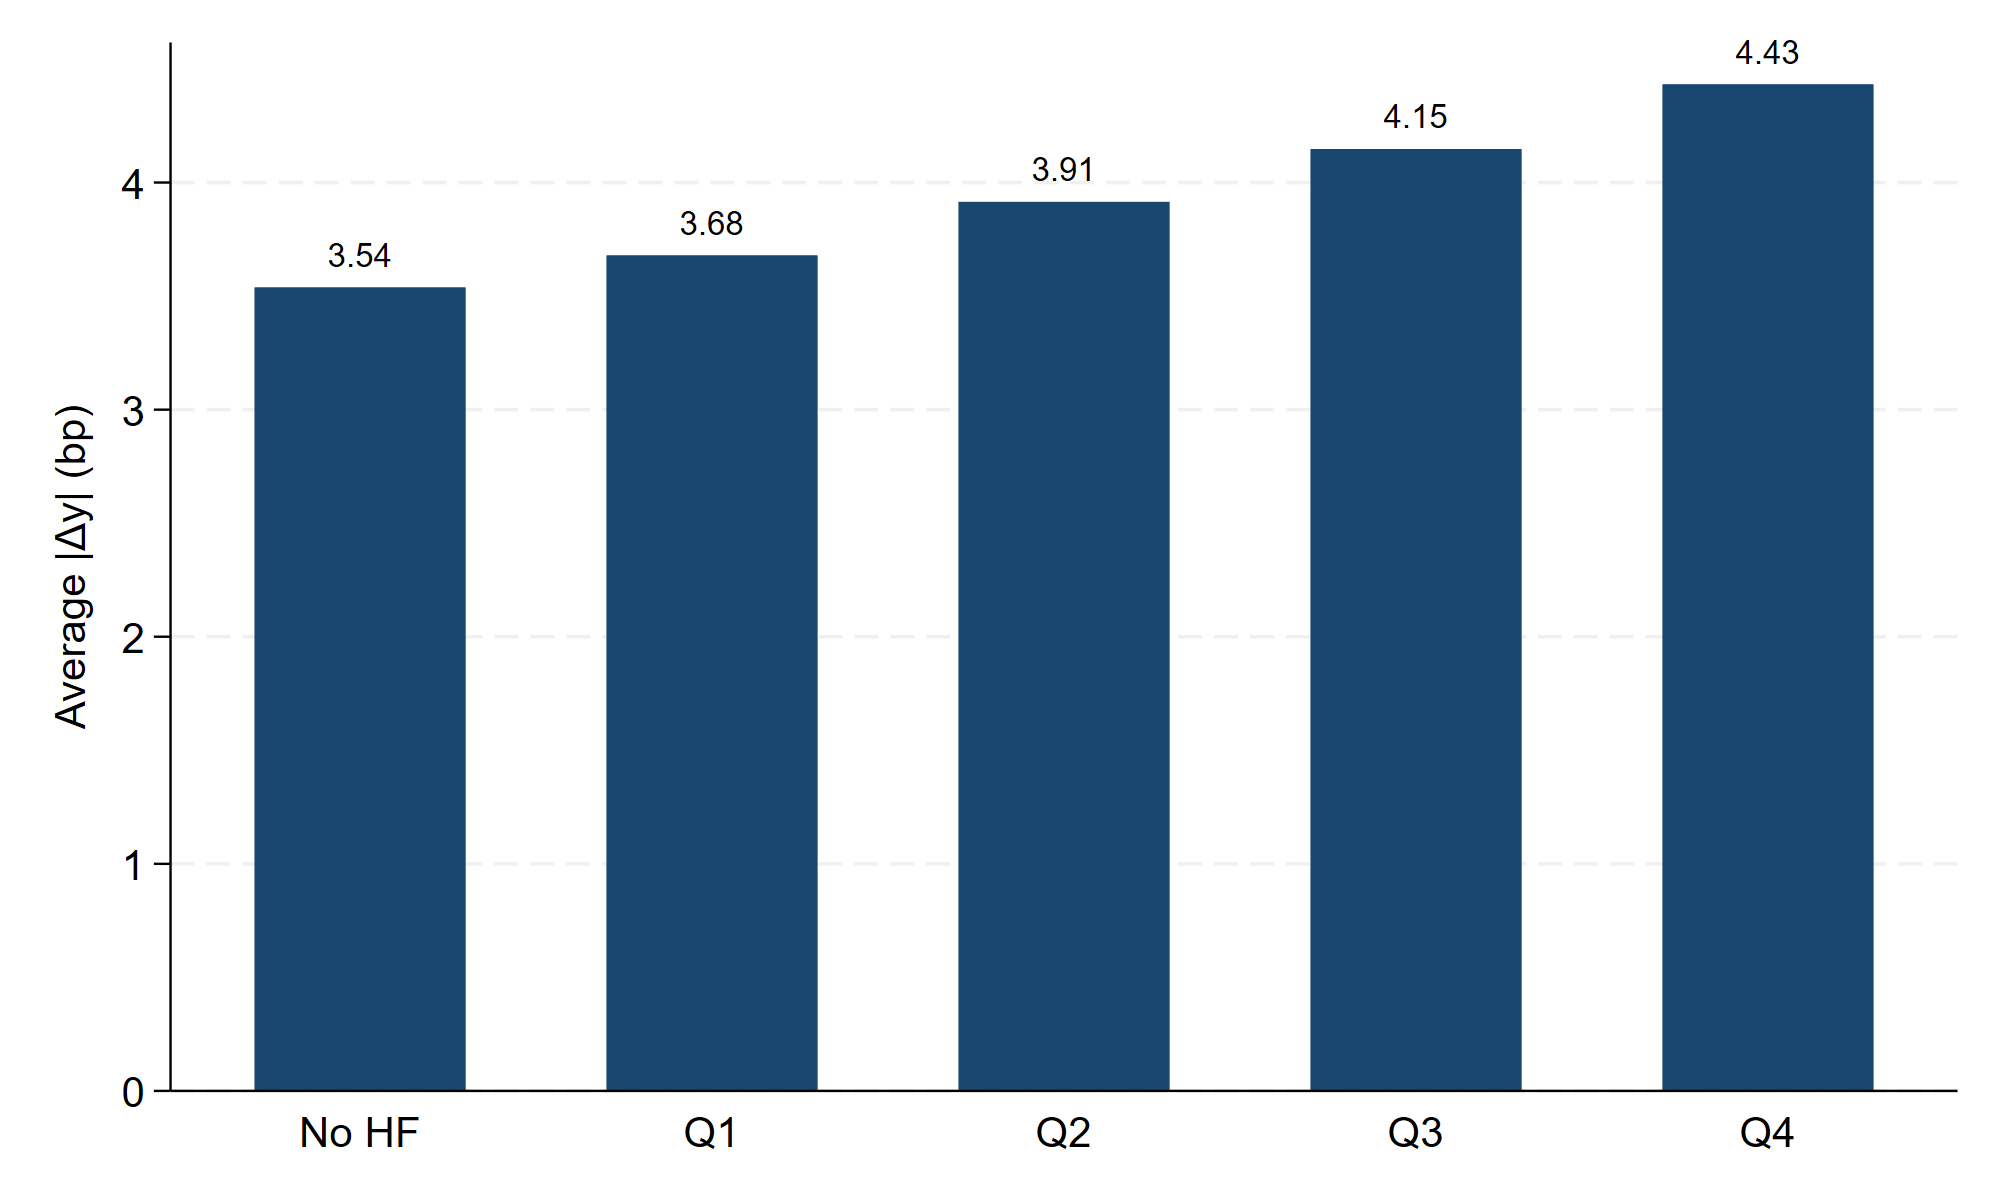
\includegraphics[width=240mm]{Figures/intensity_volatility_bars.png}
  \FigNote{Average $|\Delta$yield$|$ (bp) on non-shock days by quartile of hedge fund intensity, next to bonds without hedge funds.}
\end{minipage}\hfill
\begin{minipage}[c]{310mm}
  \fTab\centering
  \begin{tabular}{l c c}
    \toprule
    $|\Delta \text{yield}|$ (bp) & (1) Raw comparison & (2) Comparable bonds\\
    \midrule
    \textbf{HF involved $\times$ $|$Shock$|$} & \textbf{0.240}$^{***}$ & \textbf{0.246}$^{***}$\\
    HF involved (level) & 0.459$^{***}$ & $-$0.098\\
    $|$Shock$|$ & 0.545$^{***}$ & \\
    \midrule
    Bond controls & No & Yes\\
    Bond FE & No & Yes\\
    Duration $\times$ Date $\times$ Country FE & No & Yes\\
    \bottomrule
  \end{tabular}
  \FigNote{\centering Comparable bonds: similar duration, same issuer, same day.\par}
\end{minipage}

\Message{Hedge funds select volatile bonds, but the excess volatility is shock-conditional --- what changes is how yields react to shocks.}
\end{Panel}

% ============================ FINDING 2 ============================
\begin{Panel}
\Section{Finding 2: Hedge fund trading raises the sensitivity of yields to shocks}

\begin{minipage}[c]{300mm}
  \fTab\centering
  \begin{tabular}{l c c c}
    \toprule
     & \multicolumn{2}{c}{Presence} & Intensity\\
    \cmidrule(lr){2-3}\cmidrule(lr){4-4}
    $\Delta$ yield (bp) & (1) & (2) Matched & (3)\\
    \midrule
    \textbf{HF involved $\times$ Shock} & \textbf{0.291}$^{***}$ & \textbf{0.302}$^{***}$ & \\
    \textbf{HF intensity $\times$ Shock} & & & \textbf{0.164}$^{***}$\\
    HF involved (level) & $-$0.022 & $-$0.002 & \\
    HF intensity (level) & & & $-$0.011\\
    \midrule
    Bond controls & Yes & Yes & Yes\\
    Bond FE & Yes & No & Yes\\
    Duration $\times$ Date $\times$ Country FE & Yes & No & Yes\\
    Matched pair FE & No & Yes & No\\
    \bottomrule
  \end{tabular}
  \par\vspace{8mm}
  {\fStat\bfseries\color{rust}$>$\,25\%\par}\vspace{2mm}
  {\fSmall of the shock-day yield movement in hedge-fund-traded bonds reflects \textbf{positioning}, not the news itself.\par}
\end{minipage}\hfill
\begin{minipage}[c]{270mm}
  \centering
  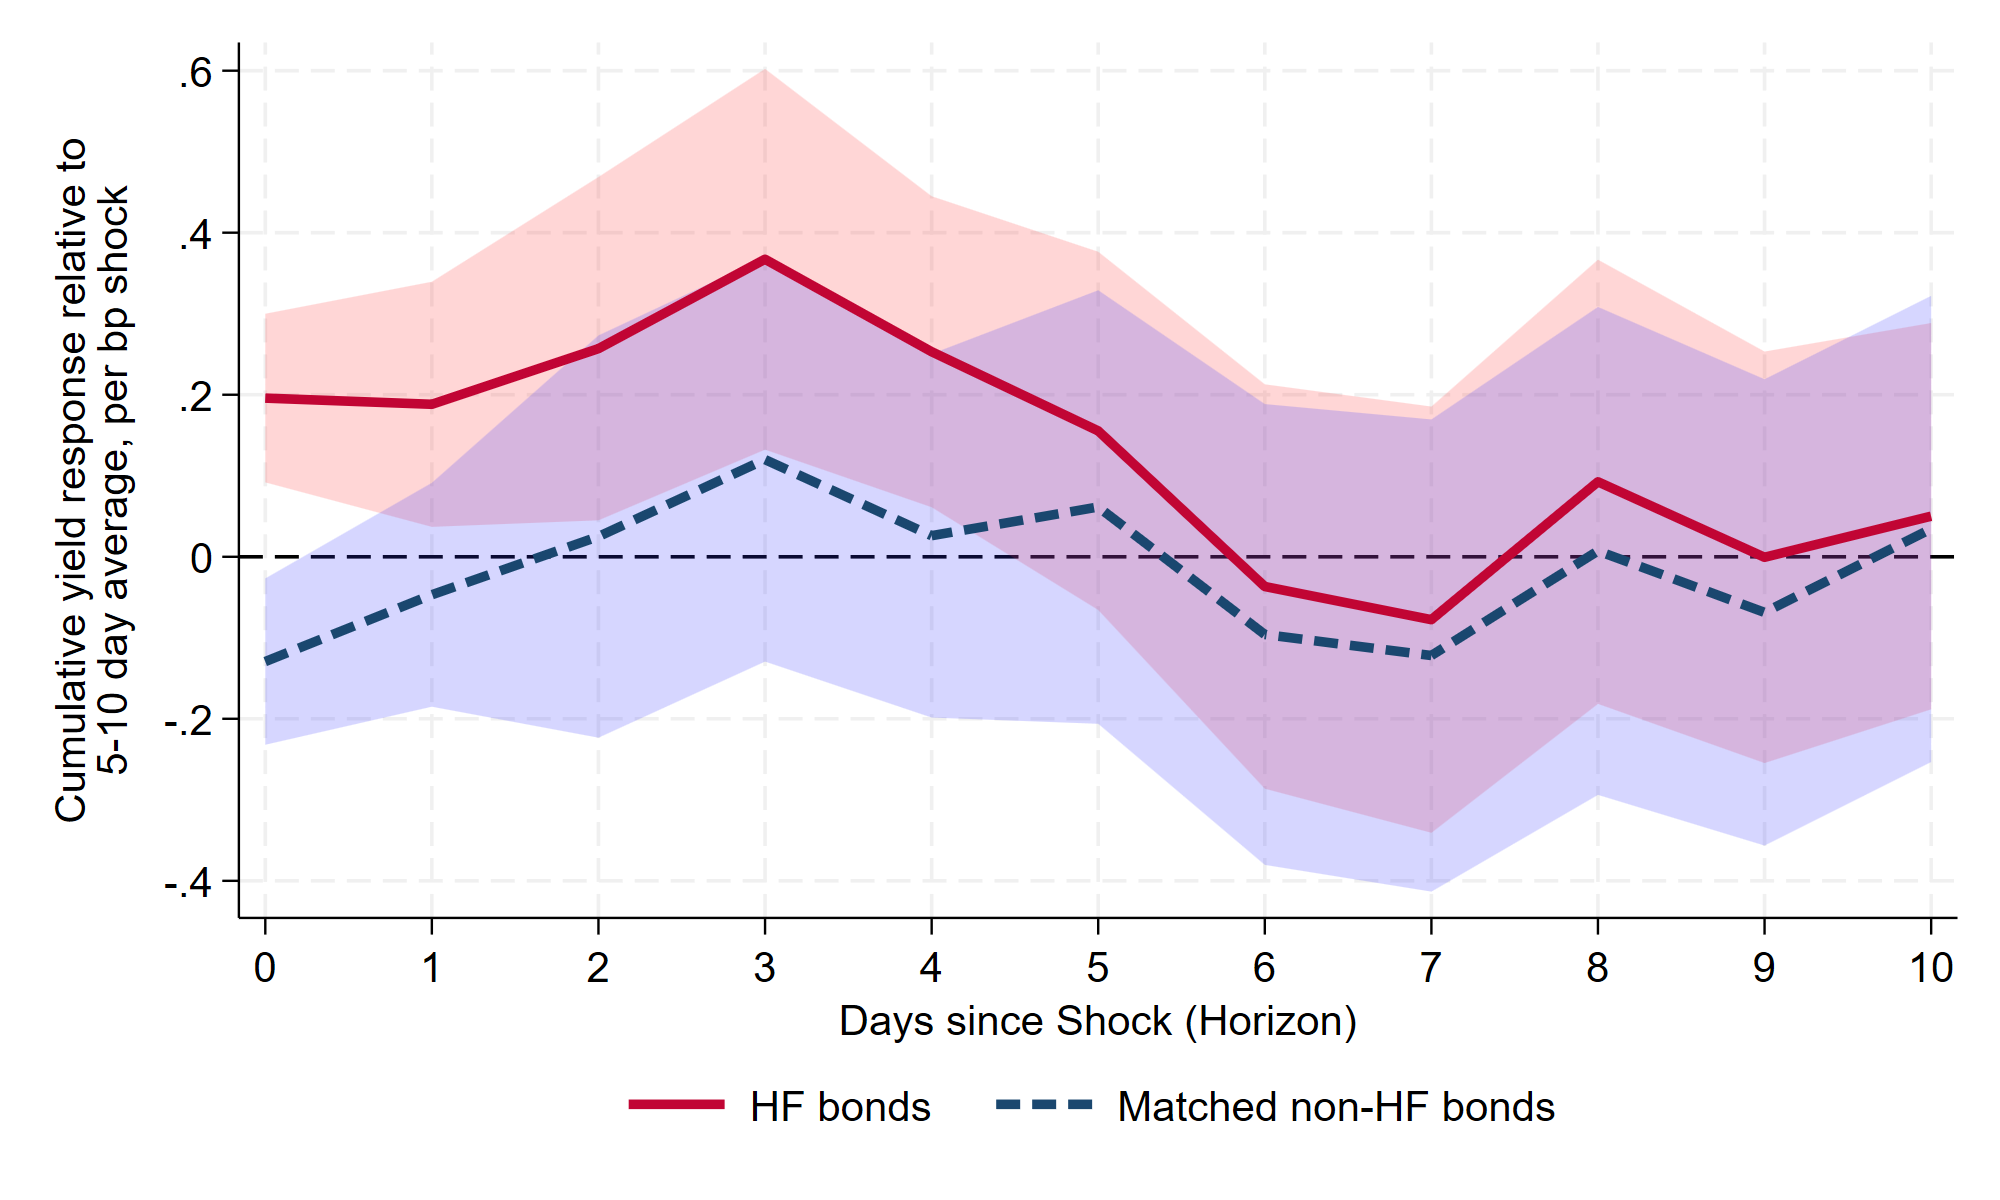
\includegraphics[width=262mm]{Figures/IR_baseline_decomposition_overshoot.png}
  \FigNote{Cumulative yield response per bp of shock, relative to the common level where both groups settle (local projections, matched sample, Jord\`a 2005). Hedge fund bonds overshoot for $\approx$\,4 days, then revert.}
\end{minipage}

\Message{Temporary overshooting that other capital gradually absorbs --- amplification, not price discovery.}
\end{Panel}

% ============================ FINDING 3 ============================
\begin{Panel}
\Section{Finding 3: The amplification holds whether shocks help or hurt the position}

\begin{minipage}[c]{280mm}
  \fTab\centering
  \begin{tabular}{l c c}
    \toprule
    $\Delta$ yield (bp) & {\color{rust}Constraining} & {\color{grn}Relaxing}\\
    \midrule
    \textbf{HF intensity $\times$ Shock} & \textbf{0.140}$^{***}$ & \textbf{0.224}$^{***}$\\
    HF intensity (level) & $-$0.016 & $-$0.009\\
    \midrule
    Bond controls & Yes & Yes\\
    Bond FE & Yes & Yes\\
    Duration $\times$ Date $\times$ Country FE & Yes & Yes\\
    \bottomrule
  \end{tabular}
  \FigNote{\centering Constraining: the shock moves against the position. Relaxing: in favor. A Wald test cannot distinguish the two ($p=0.16$).\par}
\end{minipage}\hfill
\begin{minipage}[c]{270mm}
  \centering
  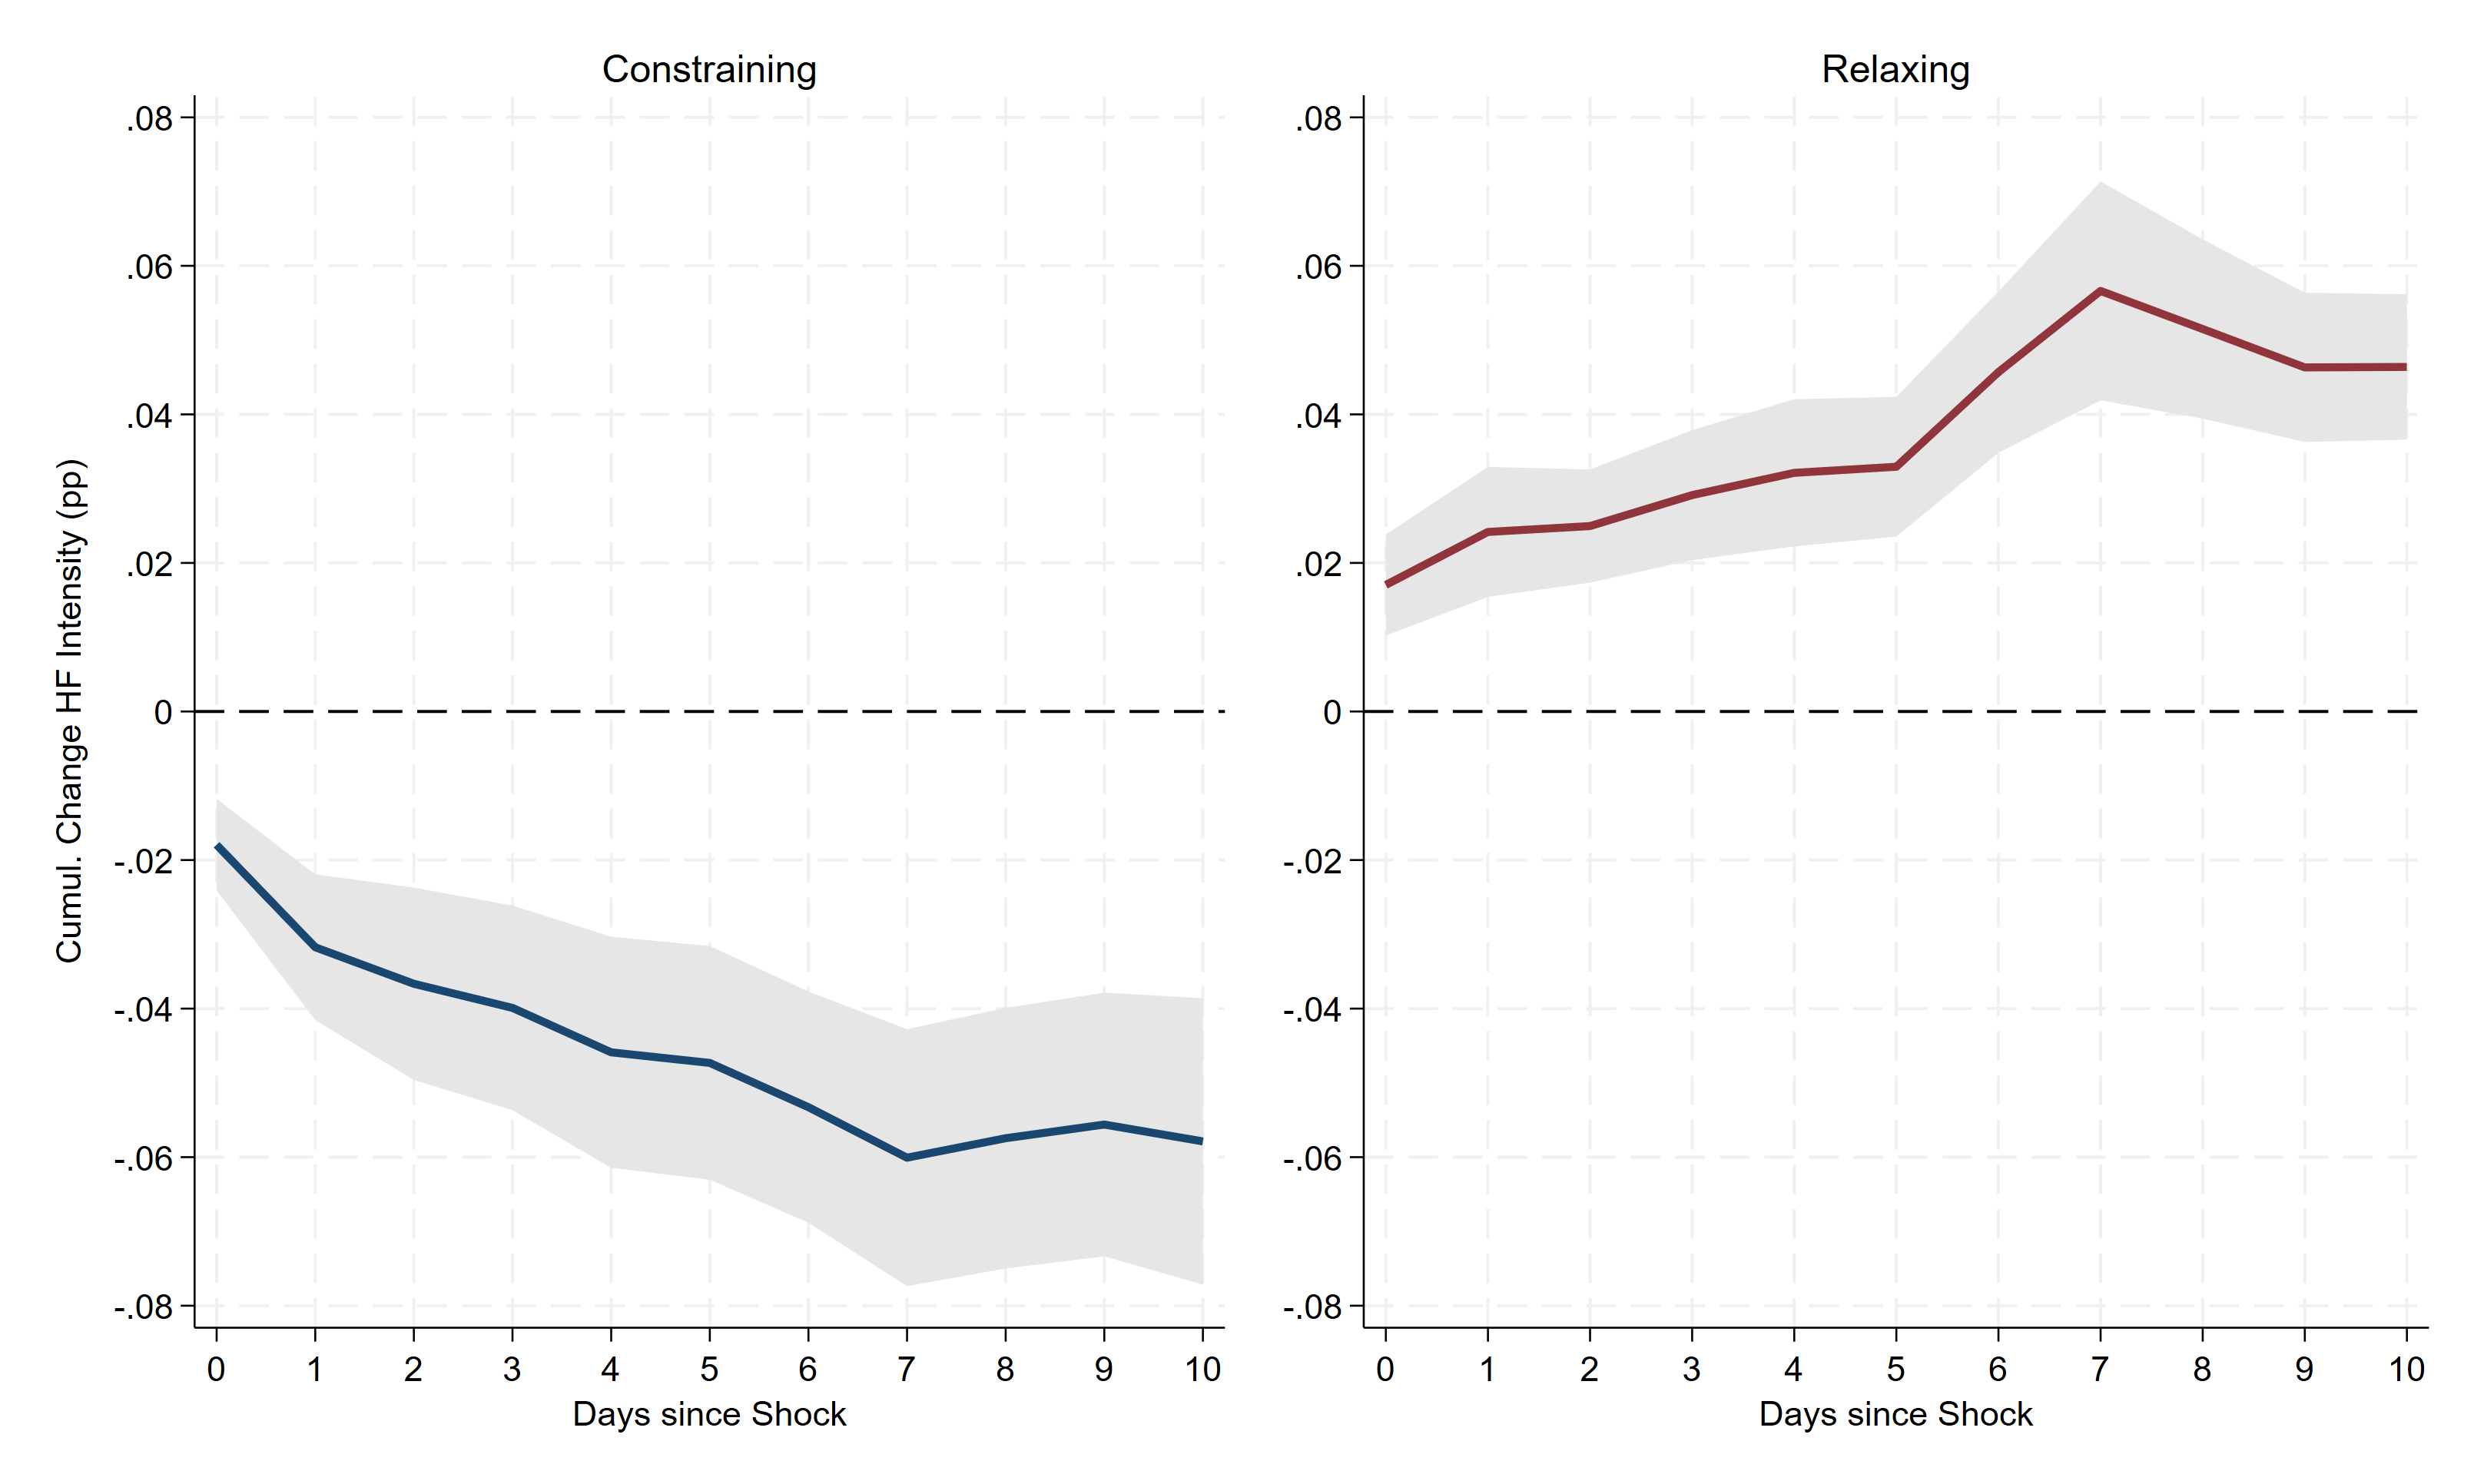
\includegraphics[width=268mm]{Figures/IR_on_momentum.png}
  \FigNote{Overnight repo positions after the shock: funds contract in the constraining regime and expand in the relaxing regime, as the mechanism predicts.}
\end{minipage}

\Message{The amplification is symmetric --- it operates whenever shocks meet positions, not only in crises.}
\end{Panel}

% ============================ FINDING 4 ============================
\begin{Panel}
\Section{Finding 4: The directionality of the book governs the strength}

\begin{minipage}[c]{272mm}
  \centering
  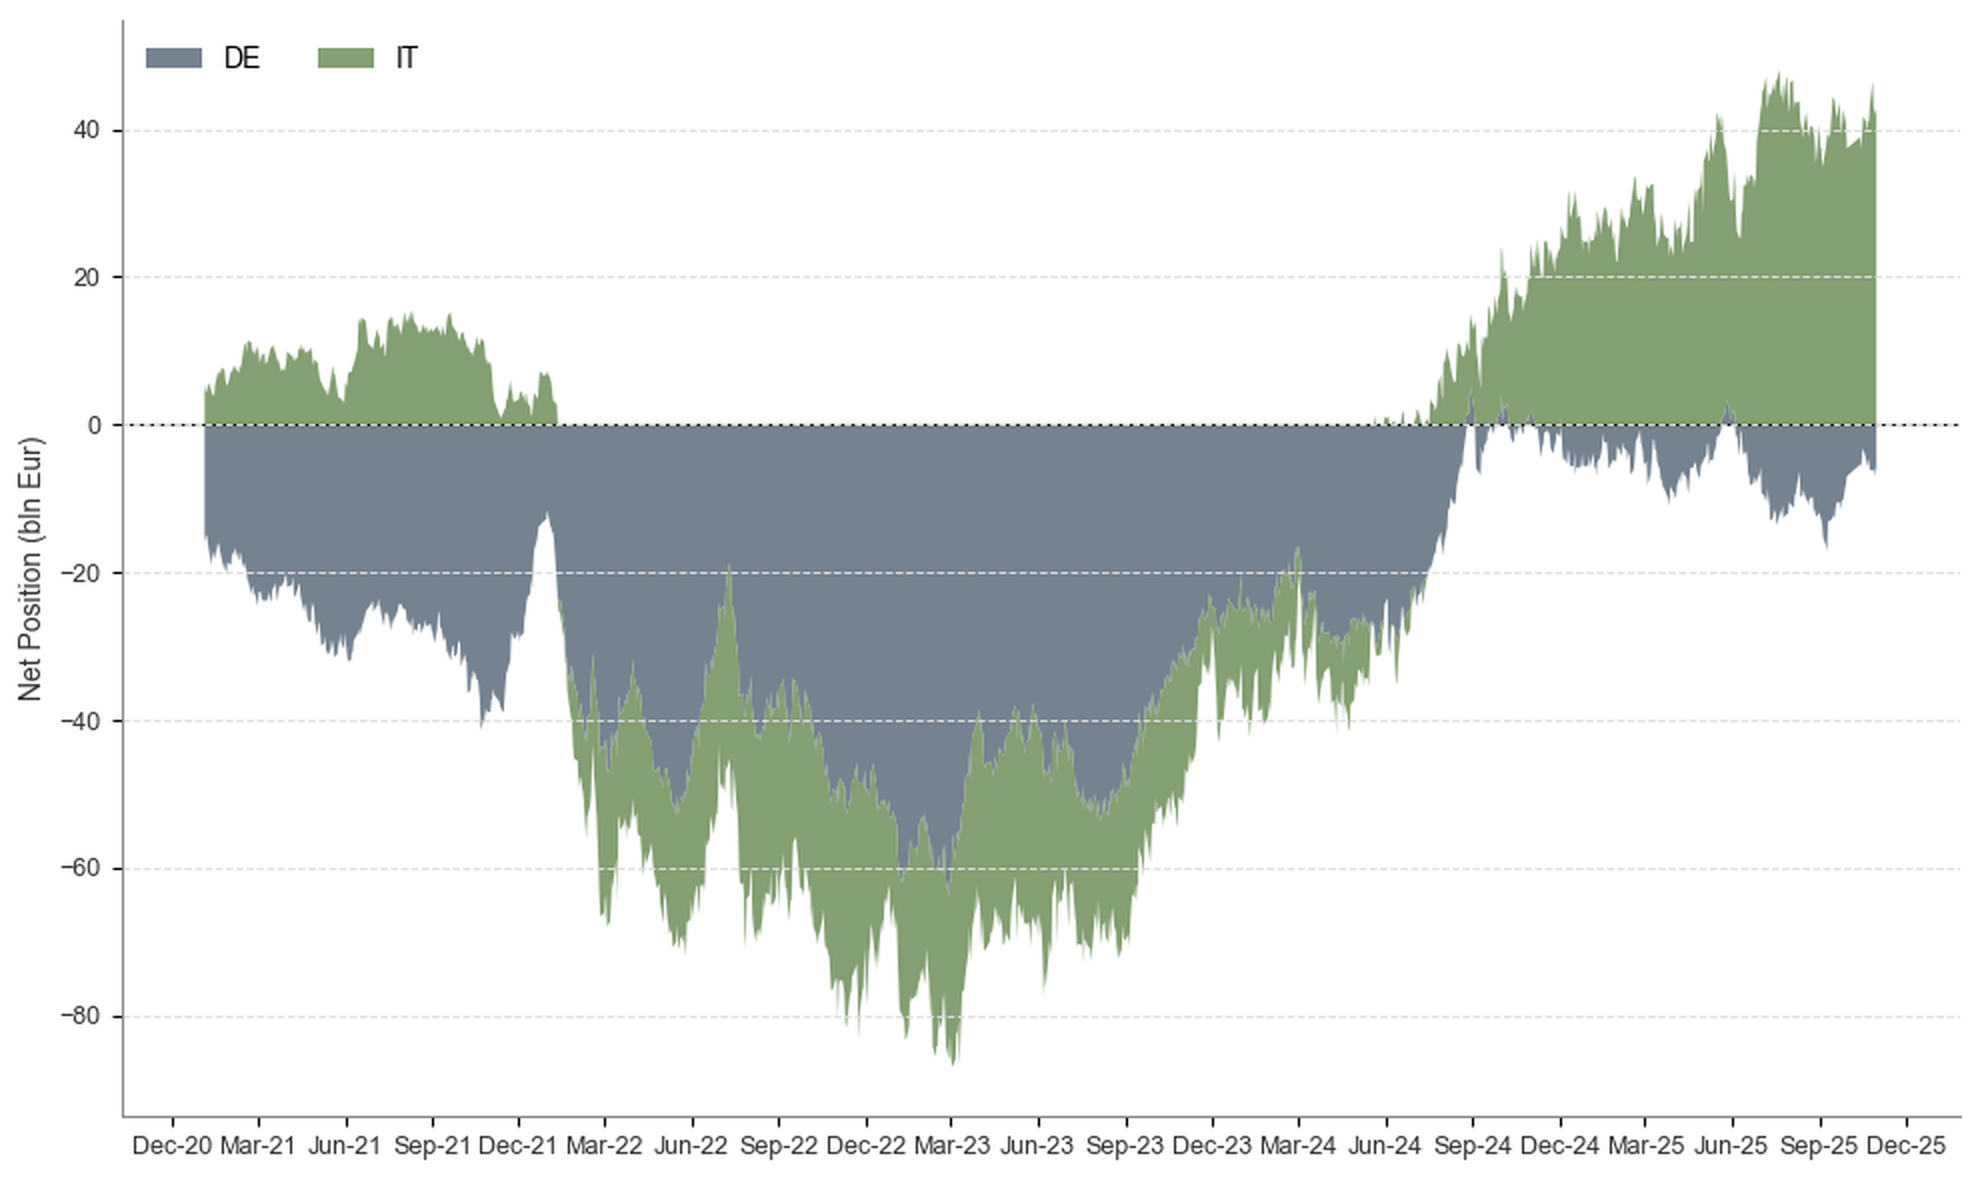
\includegraphics[width=264mm]{Figures/motivation_chart.png}
  \FigNote{Aggregate net repo positions in German (DE) and Italian (IT) sovereigns. Around the hiking cycle: long IT, short DE (hedged book). During it: one-sided short (directional book).}
\end{minipage}\hfill
\begin{minipage}[c]{300mm}
  {\fBody A fund manages one pool of capital: a duration-hedged book barely loses capital on a level move, a directional book absorbs the full hit.\par}
  \vspace{6mm}
  \fTab\centering
  \begin{tabular}{l c}
    \toprule
    $\Delta$ yield (bp), relative to no HF & Coefficient\\
    \midrule
    Hedged book $\times$ Shock & 0.098$^{***}$\\
    \textbf{Directional book $\times$ Shock} & \textbf{0.363}$^{***}$\\
    \midrule
    Q1 most hedged $\times$ Shock & 0.057\\
    Q2 $\times$ Shock & 0.137$^{***}$\\
    Q3 $\times$ Shock & 0.361$^{***}$\\
    \textbf{Q4 most directional $\times$ Shock} & \textbf{0.367}$^{***}$\\
    \bottomrule
  \end{tabular}
  \FigNote{\centering Bond and duration $\times$ country $\times$ date FE with controls. Wald tests reject equality of the hedged and directional groups ($F=24.8$) and of the extreme quartiles ($F=28.3$).\par}
\end{minipage}

\Message{The amplification rises monotonically with directionality and vanishes when the book is hedged.}
\end{Panel}

% ========================= CONCLUSION =========================
\begin{Panel}
\Section{Conclusion: what this means for risk monitoring}

\begin{minipage}[t]{300mm}\fBody
\begin{itemize}
  \item \textbf{More than a quarter} of the shock-day yield move reflects positioning; it reverts within days.
  \item The amplification is \textbf{symmetric} across constraining and relaxing states.
\end{itemize}
\end{minipage}\hfill
\begin{minipage}[t]{300mm}\fBody
\begin{itemize}
  \item It is \textbf{not confined to stress episodes}.
  \item The \textbf{\color{rust}directionality} of the book is the key risk metric beyond position size.
\end{itemize}
\end{minipage}
\end{Panel}

\vfill

% ============================= FOOTER =============================
\fullbleed{%
\begin{tcolorbox}[colback=navy,colframe=navy,sharp corners,boxrule=0pt,
    width=710mm,left=50mm,right=50mm,top=10mm,bottom=24mm]
  \color{white}\centering
  {\fSub\bfseries Felix Hermes\par}
  \vspace{2mm}
  {\fBody Goethe University Frankfurt \& European Central Bank \hspace{1.5em}$\cdot$\hspace{1.5em} hermes@finance.uni-frankfurt.de\par}
\end{tcolorbox}}

\end{document}
